\section{Foreword}
\subsection{}

\begin{frame}
\frametitleTC{Direct synthesis -- choosing $G_{yw}^{\circ}$ and $G_{yd}^{\circ}$}
\framesubtitleTC{The ideal selection}
\myPause
 \begin{center}
  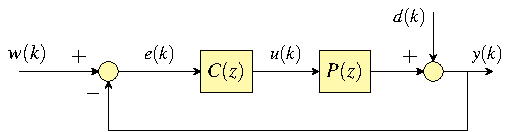
\includegraphics[width=0.50\columnwidth]{./Unit-04/img/ControlLoop-H1.pdf}
 \end{center}\myPause
 \begin{itemize}[<+-| alert@+>]
 \item If possible, we would like to have
       \begin{displaymath}
        G_{yw}^{\circ}(z) = \frac{1-\alpha}{z-\alpha}, \quad
        G_{yd}^{\circ}(z) = \frac{z-1}{z-\alpha}, \qquad
        0 < \alpha < 1.
       \end{displaymath}
 \item The reason is that this gives the best tracking of a step set point\\
       variation, and the best rejection of a step disturbance. 
 \end{itemize}
\end{frame}

\begin{frame}[fragile]
\frametitleTC{Direct synthesis -- choosing $G_{yw}^{\circ}$ and $G_{yd}^{\circ}$}
\framesubtitleTC{The ideal selection}
\myPause
 \begin{itemize}[<+-| alert@+>]
 \item What do we mean ``best''?
 \item Try in Scilab some values of $\alpha$, say 0.1, 0.5 and 0.9, and plot the corresponding\\
       step responses:
       {\scriptsize
       \begin{verbatim}
     Gyw = syslin('d',(1-0.5)/(%z-0.5)); // Example with alpha=0.5
     Gyd = syslin('d',(%z-1)/(%z-0.5));
     wd  = ones(1,20);                   // Step inputs (w for Gyw, d for Gyd)
     yw  = dsimul(tf2ss(Gyw),wd); 
     yd  = dsimul(tf2ss(Gyd),wd); 
     plot(yw,'b');                       // Response of Gyw in blue
     plot(yd,'r');                       // Response of Gyd in red
       \end{verbatim}
       }
 \item \vspace{-4mm}Comments:
       \begin{itemize}[<+-| alert@+>]
       \item exact asymptotic tracking of $w$, no overshoot, no oscillations;
       \item exact asymptotic rejection of $d$, monotonic response;
       \item the one parameter $\alpha$ governs tracking/rejection speed, namely\\
             $\alpha\rightarrow 0 \Rightarrow$ faster (\TC{``fast pole''}),\\
             $\alpha\rightarrow 1 \Rightarrow$ slower (\TC{``slow pole''}).
       \end{itemize}
 \item Are there alternatives? Yes --- come to advanced control courses \smiley.
 \end{itemize}
\end{frame}
